\documentclass{sigchi}

% Use this command to override the default ACM copyright statement (e.g. for
% preprints).
% Consult the conference website for the camera-ready copyright statement.

%% EXAMPLE BEGIN -- HOW TO OVERRIDE THE DEFAULT COPYRIGHT STRIP
%% (July 22, 2013 - Paul Baumann)
\toappear{LIDET is located inside the Department of Computer Science of the
          Institute of Mathematics and Statistics, at the University of S\~ao
          Paulo\\
          Rua do Mat\~ao, 1010, CEP 05508-090, S\~ao Paulo, SP, Brazil\\
          Telephone: +55 11 3091--9600\\

          Daros is a MSc student, Vieira and Pereira are PhD students, and
          Corr\^ea da Silva is their advisor.\\

          This manuscript was submitted in November 21st 2014 to the iGAM4ER
          2014 competition (http://igam4er.org/) taking place in Paris, France,
          in December 13th and 14th 2014.
}
%% EXAMPLE END -- HOW TO OVERRIDE THE DEFAULT COPYRIGHT STRIP
%% (July 22, 2013 - Paul Baumann)

% Arabic page numbers for submission.
% Remove this line to eliminate page numbers for the camera ready copy
% \pagenumbering{arabic}

% Load basic packages
\usepackage{balance}  % to better equalize the last page
\usepackage{graphics} % for EPS, load graphicx instead
\usepackage{times}    % comment if you want LaTeX's default font
\usepackage{url}      % llt: nicely formatted URLs
\usepackage{tabu}
\usepackage{subcaption}
\usepackage{enumitem}
\usepackage{multicol}

\usepackage{enumitem}

% llt: Define a global style for URLs, rather that the default one
\makeatletter
\def\url@leostyle{%
    \@ifundefined{selectfont}{\def\UrlFont{\sf}}{%
        \def\UrlFont{\small\bf\ttfamily}%
    }}
\makeatother
\urlstyle{leo}

% To make various LaTeX processors do the right thing with page size.
\def\pprw{8.5in}
\def\pprh{11in}
\special{papersize=\pprw,\pprh}
\setlength{\paperwidth}{\pprw}
\setlength{\paperheight}{\pprh}
\setlength{\pdfpagewidth}{\pprw}
\setlength{\pdfpageheight}{\pprh}

% Make sure hyperref comes last of your loaded packages,
% to give it a fighting chance of not being over-written,
% since its job is to redefine many LaTeX commands.
\usepackage[pdftex]{hyperref}
\hypersetup{
    bookmarksnumbered,
    pdfstartview={FitH},
    colorlinks,
    citecolor=black,
    filecolor=black,
    linkcolor=black,
    urlcolor=black,
    breaklinks=true,
}

% create a shortcut to typeset table headings
\newcommand\tabhead[1]{\small\textbf{#1}}

% path of images
\graphicspath{{./images/}}

% Shared affiliations
\def\sharedaffiliation{%
\end{tabular}
\begin{tabular}{c}}

% To keep the url in the same font of the institution address
\newcommand{\urlwofont}[1]{\urlstyle{same}\url{#1}}

% Column types for text
\newcolumntype{L}[1]{>{%
    \raggedright\let\newline\\\arraybackslash\hspace{0pt}}m{#1}%
}
\newcolumntype{C}[1]{>{%
    \centering\let\newline\\\arraybackslash\hspace{0pt}}m{#1}%
}
\newcolumntype{R}[1]{>{%
    \raggedleft\let\newline\\\arraybackslash\hspace{0pt}}m{#1}%
}

\newcommand{\refsectitle}[1]{\ref{#1}~(\nameref{#1})}

% End of preamble. Here it comes the document.
\begin{document}

% Define the name of the game
\newcommand{\rawgamename}{Sweet Switches}
\newcommand{\rawgamenamept}{Sabores Seletos}
\newcommand{\gamename}{\textbf{\emph{\rawgamename}}}
\newcommand{\gamenamept}{\textbf{\emph{\rawgamenamept}}}

\newcommand{\doctorgame}{\emph{The Doctor and the Dalek}}
\newcommand{\labview}{\emph{LabVIEW}}
\newcommand{\scratch}{\emph{Scratch}}
\newcommand{\codecombat}{\emph{CodeCombat}}
\newcommand{\manufactoria}{\emph{Manufactoria}}
\newcommand{\lightbot}{\emph{Lightbot}}

\newcommand{\doctorsite}{\url{http://en.wikipedia.org/wiki/Dalek}}
\newcommand{\mindstormsite}{\url{http://mindstorms.lego.com}}
\newcommand{\scratchsite}{\url{http://scratch.mit.edu/}}
\newcommand{\manufactoriasite}{\url{http://pleasingfungus.com/Manufactoria/}}
\newcommand{\excelsite}{\url{http://office.microsoft.com/excel}}
\newcommand{\lightbotsite}{\url{http://lightbot.com/hocflash.html}}

\title{\rawgamename: a Digital Game to Foster Learning Computer Programming
       Skills}

\numberofauthors{4}
\author{
    \alignauthor Vin\'icius Kiwi Daros\\
        \email{vkdaros@ime.usp.br}
%
    \alignauthor Luiz Carlos Vieira\\
        \email{lvieira@ime.usp.br}
%
    \alignauthor Adalberto Bosco C. Pereira\\
        \email{bosco@ime.usp.br}
%
    \alignauthor Fl\'avio S. Corr\^ea da Silva\\
        \email{fcs@ime.usp.br}
%
    \sharedaffiliation
        \affaddr{Laboratory of Interactivity and Digital Entertainment%
                 Technology (LIDET)}\\
        \affaddr{\urlwofont{http://www.ime.usp.br/~lidet}}
}
\maketitle

\begin{abstract}
    Computers first uses were restricted to a small number of people, but this
    scenario has changed drastically and they become a huge part of modern life.
    Although there is an effort to bring computers to basic educational program,
    the approach currently in use hasn't been effective. In order to increase
    the interest of students in this subject and introduce programming concepts
    without forcing code writing, we present \gamename. In this game the student
    will face a series of puzzles inside ice cream factories. The objective is
    to attach devices to conveyors belt in order to attend a production request.
    Those devices are analogous to programming statements. Although playing the
    game will not teach students to write computer programs, it will help them
    to develop skills useful for solving computer problems.
\end{abstract}

\keywords{
    games; education; computer programming; logical thinking; Brazilian fauna
}

\category{K.3.1.}{Computer Uses in Education}{Computer-assisted instruction%
                  (CAI)}
\category{K.8.0.}{Personal Computing}{Games}

\section{Introduction}
    In all developed countries, primary school children have at least one class
    a week when they use a computer \cite{Istrate2010}, but so far computers
    have been mostly employed to aid in other disciplines and as a productivity
    tool. So that it has been argued that young people should be educated not
    only in the application and use of technology, but also in
    \textit{how it works} and what are its \textit{fundamental principles}. A
    report prepared for the UK Computing Research Committee \cite{Jones2009}
    particularly mentions the fact that UK students are now becoming
    disenchanted with the computer aided learning because they arrive at school
    with a much richer background in ICT (Information and Communication
    Technology) then early students. The report also advocates that if on one
    hand learning how to use computers can be seen as similar to learning how to
    read, on the other hand learning how to program computers is similar to
    learning how to write. They are both skills that everyone should have, even
    though only a minority will become professionals (writers or computer
    programmers).

    Despite grounded arguments both in favor and against the use of computers by
    children \cite{Istrate2010,Setzer2001} and the relevance of the so called
    ``computer literacy'' or ``computational thinking'' trend
    \cite{Wing2006,Atwood2012}, the study of computer programming elements at
    primary and secondary school is increasingly being acknowledged as equally
    important as other disciplines such as math or science. The main reason is
    that the skills required for programming computers are definitely valuable
    for education, since they involve procedural thinking, problem solving
    through trial and error, creativity, thinking about thinking, and the
    analysis and exploration of data \cite{Kahn1999}.

    The experience the authors of this paper have had in teaching basic computer
    programming at the graduation course in Administration at the University of
    S\~ao Paulo corroborates that even when employing tools that the students
    are required to use in their daily routines and are accustomed with -- such
    as the Microsoft Office Excel\footnote{\excelsite} with the Visual Basic for
    Applications (VBA) programming language -- the task of learning how to use
    control structures in planning and solving problems by iterative execution
    is still perceived as a tedious activity even for older students.

    As consequence, the authors have been working on the development of a
    digital game called \gamename~(\gamenamept~in Portuguese), which has
    educational intentions mainly related to the development of skills necessary
    for programming computational tasks, \textit{but not directly involving
    coding}. The game mechanics is based on planning and building a production
    line that gets increasingly more complex as the player improves his or her
    understanding of how the control flow works. The next sections will describe
    existing similar playful environments and games that served as inspiration
    and details of the game under development.

\section{Similar Existing Products}
    Using games as teaching tool is not novelty. There are many good examples of
    games with this purposes and they were inspiration for our project. In this
    section we describe a few games somehow related to computing education and
    group them in three categories.

    \subsection{Playful Environments used for Teaching Programming}
        Playful environments employed to teach programming to children usually
        rely on motivating the creation of code from fun interactions with the
        real world or by allowing children to create their own content. One of
        the first examples of these environments is \labview \cite{Erwin2000},
        used to help programing the behaviors of robots made of modular sensors
        and motors in the LEGO Mindstorms\footnote{\mindstormsite}. It is a
        visual interface in which programs are built by stringing basic
        subroutines together in a block diagram, which can then be further
        reused as a new routines in higher levels.

        Another very popular example of playful environment is MIT's
        \scratch\footnote{\scratchsite} \cite{Resnick2009}. It is also a visual
        tool composed of graphical blocks that children snap together to move
        images or play sounds. The format of these blocks are carefully designed
        so they intuitively indicate syntax restrictions. For instance, a
        decision block (the ``if'' yellow block at figure~\ref{fig:scratch}) is
        C-shaped to suggest that other blocks can fit inside it.

    %\subsection{Games used for Teaching Sequential and Logical Thinking}
    \subsection{Teaching Sequential and Logical Thinking with Games}
        % We should mention LightBot.
        There are also games used for teaching programming, but instead of
        allowing a free test-bed environment they are games that involve
        computer programming in the mechanics. One famous example is \codecombat 
        \cite{Saines2013}. This is an adventure game in which players control
        the hero character indirectly by programing behaviors through coding
        small functional actions such as move right, left, down and up, find
        nearest enemy and attack enemy. The game allows coding in many different
        programming languages, and includes important concepts like use of
        variables and repetition blocks.

        A very recent example is BBC's \doctorgame \cite{BBC2014}. This is a
        platform game in which the player directly controls a Dalek
        cyborg\footnote{\doctorsite}, an extraterrestrial race from the British
        science fiction series \textit{Doctor Who}. The programming is used in
        the fantasy of the game as a manner of improving the cyborg abilities at
        the end of completed levels, like programming its jump or attack
        behaviors (as illustrated in figure~\ref{fig:dr-who}).

        \begin{figure}
            \centering
            \begin{subfigure}[!h]{0.5\columnwidth}
                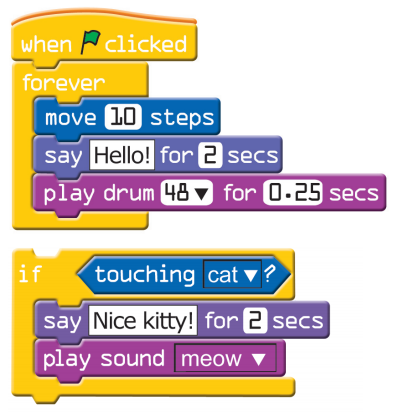
\includegraphics[width=\textwidth]{scratch}
                \caption{Sample programs from \scratch}
                \label{fig:scratch}
            \end{subfigure}%

            \begin{subfigure}[!h]{0.7\columnwidth}
                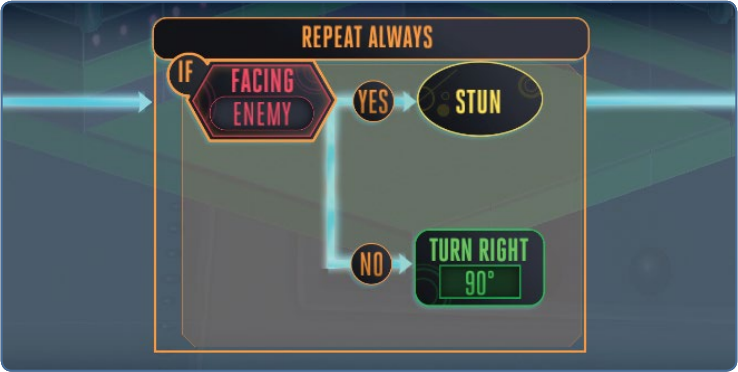
\includegraphics[width=\textwidth]{dr-who}
                \caption{Repetition block from a program in Dr. Who and the
                         Dalek}
                \label{fig:dr-who}
            \end{subfigure}
            \caption{Programming in playful environments and games}
            \label{fig:samples}
        \end{figure}

    \subsection{Games involving Logistics}
        There are many games involving logistics, that is the management of the
        flow of resources between points to meet some requirements. One title
        worth mention is \manufactoria \footnote{\manufactoriasite}. As
        \gamename, that game also has a factory scenario. But the most important
        similarity is the indirect approach of teaching computing concepts.

        In \manufactoria, players must place conveyor tiles and switches on a
        grid. The objective is to guide a robot from the ``input gate'' to the
        ``accepted gate'' only if the robot's label has the correct sequence of
        colors. The puzzle mechanic is basically the same of an automaton
        consuming an string and accepting or rejecting it. Each level presents
        classical automaton problems, such as only accepting strings which
        starts and finishes with the same color (character).

        The analogy is evident to computer scientists but the game succeeds to
        expose automaton concepts and challenges sparing players the ``scary''
        name and formalisms. This is very close to our goal with \gamename: to
        make a game that is truly perceived as a game but in the same time is a
        tool to develop and evolve procedural thinking skills.

\section{The \gamename\ Project}
    \gamename is a puzzle game in which the player needs to build an ice cream
    factory by correct placing cup dispensers, flavor and topping dosers, path
    switchers and other devices on a predefined layout of conveyors, in order to
    produce different types of ice creams in the requested quantities by
    customers.

    % This concept art images are ``misplaced'' here because otherwise they were
    % showing up only after References.
    \begin{figure*}
        \centering
        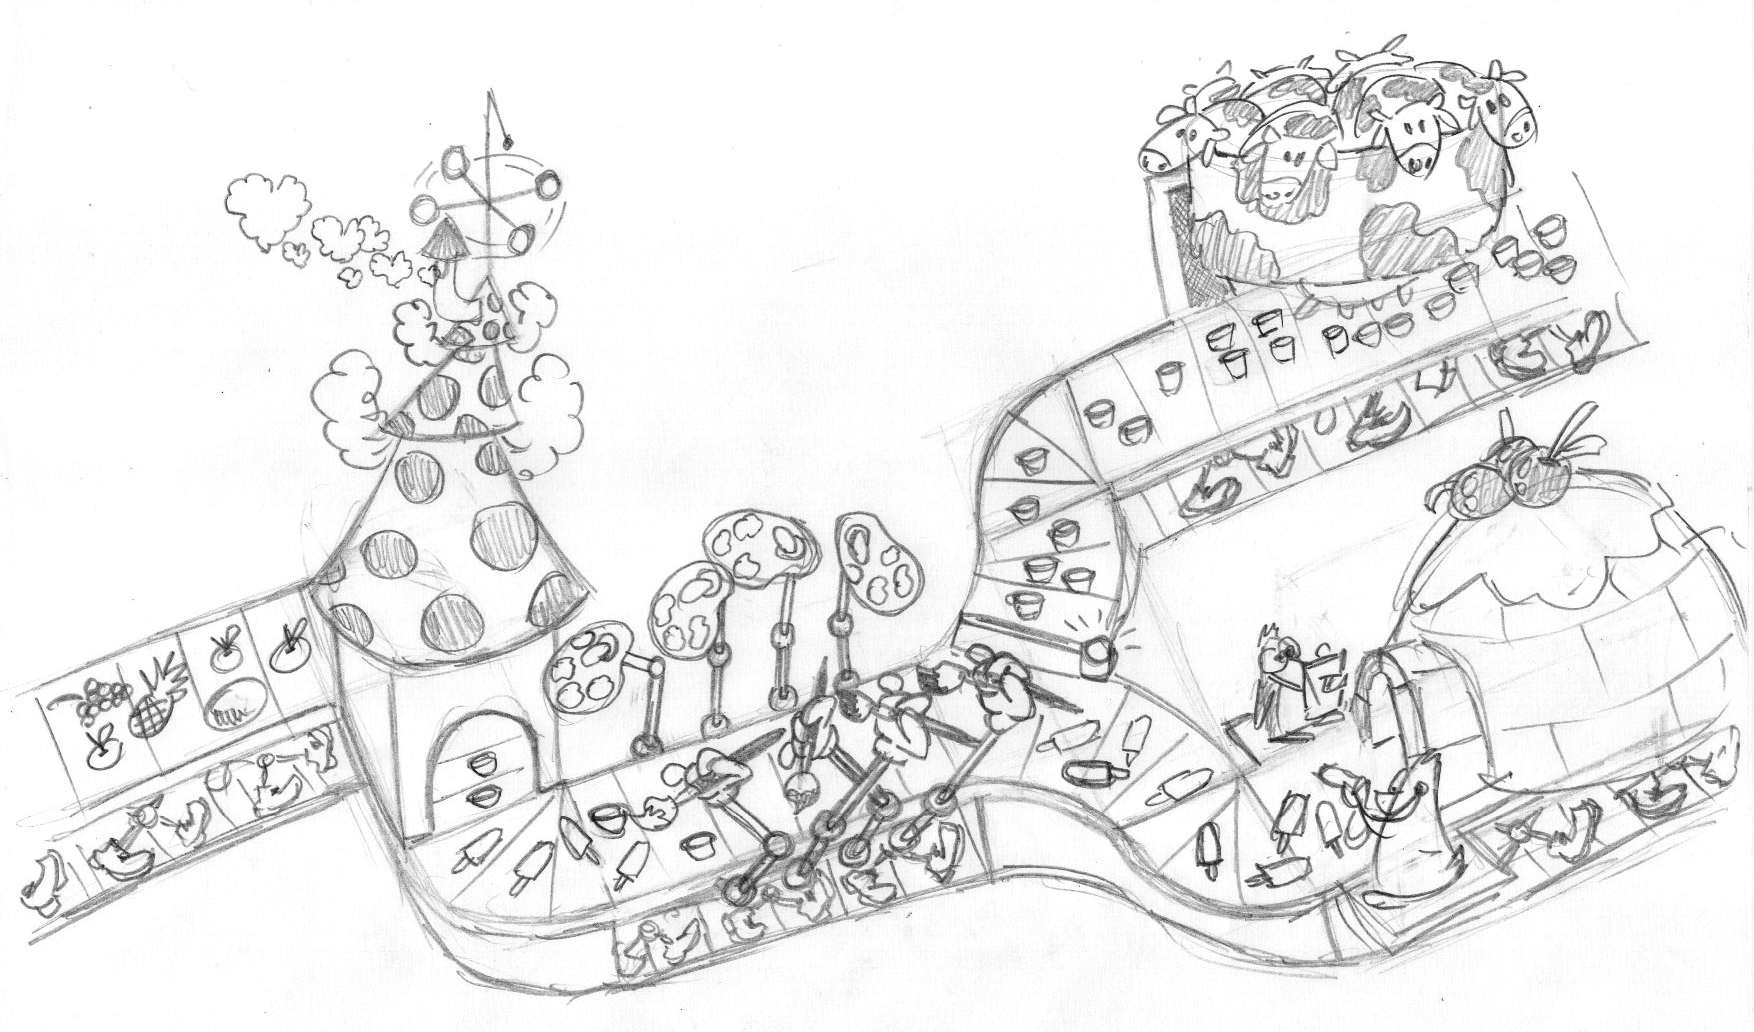
\includegraphics[height=12em]{01}
        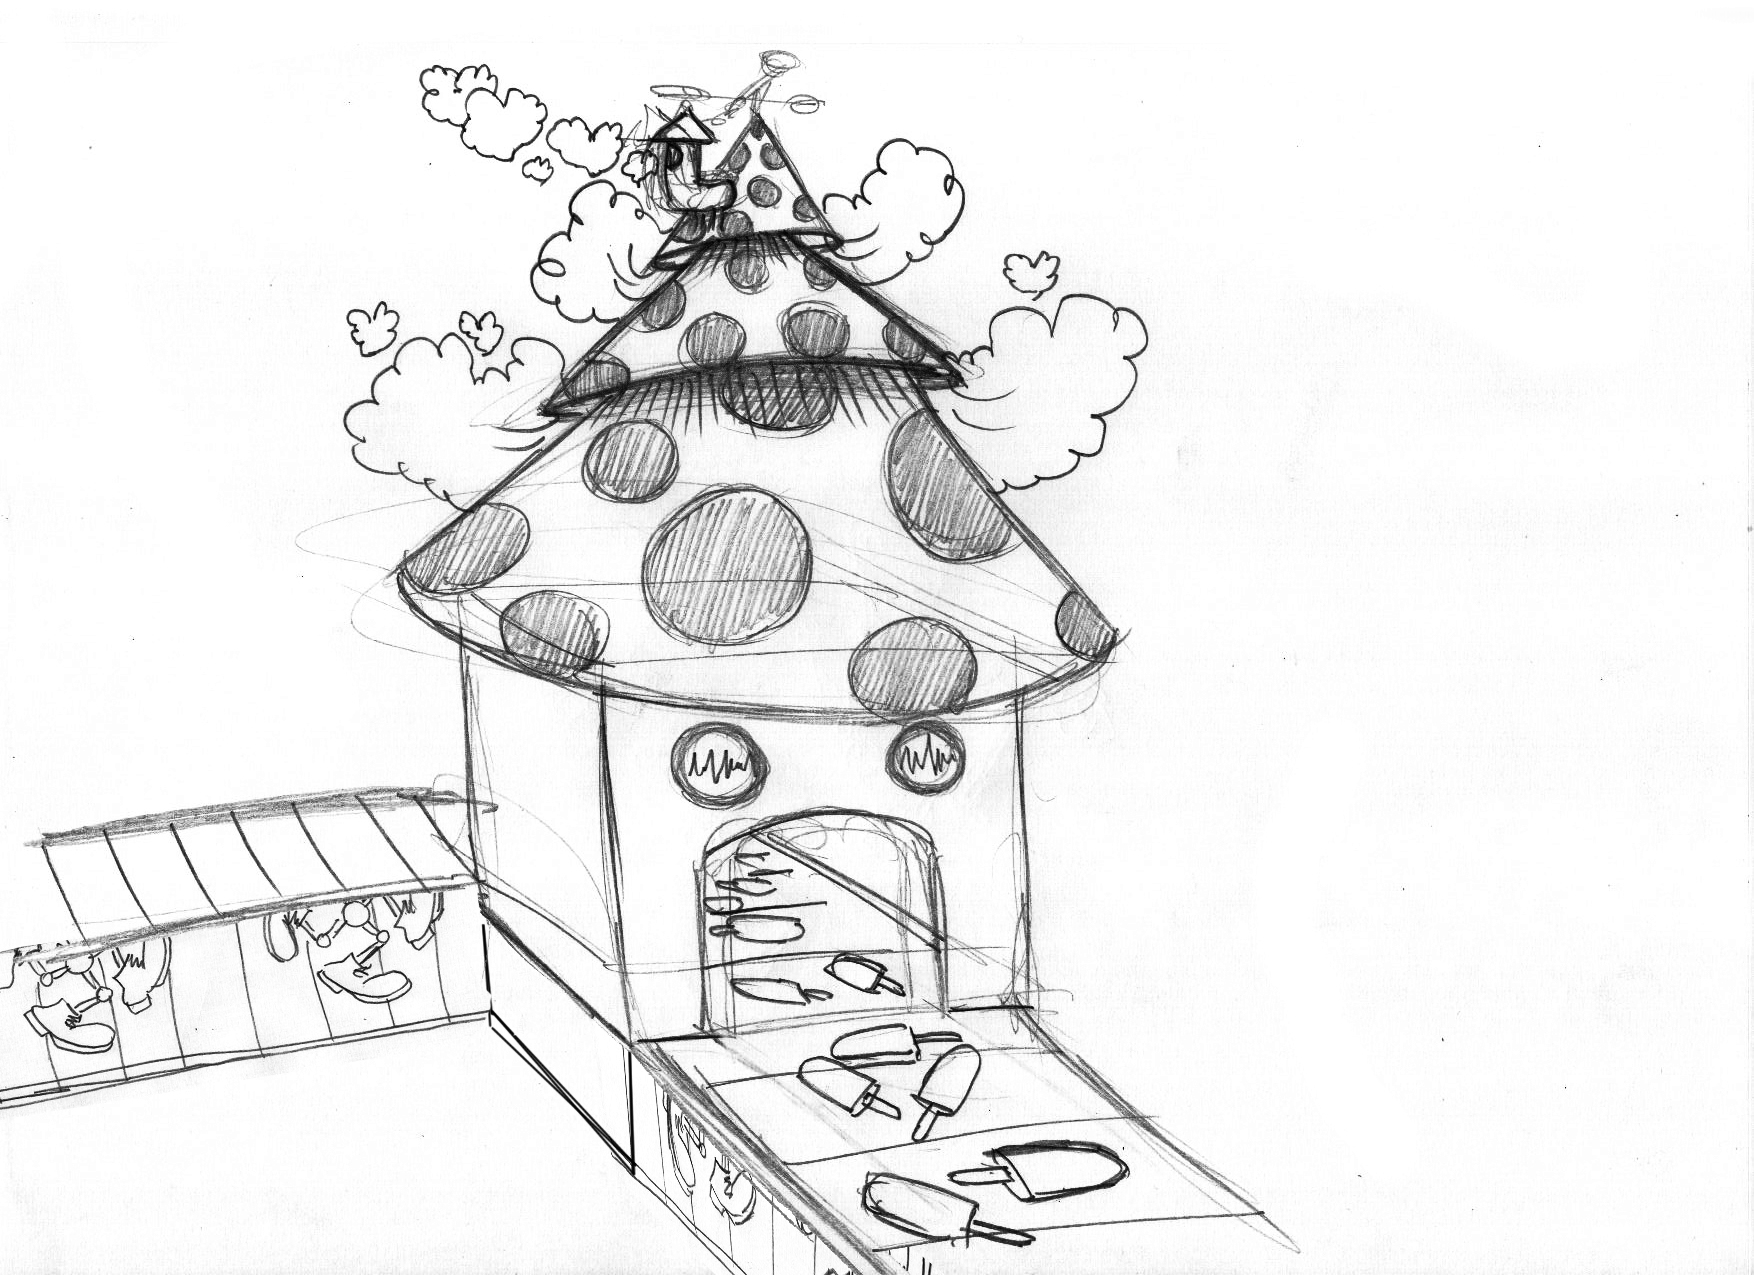
\includegraphics[height=12em]{02}
        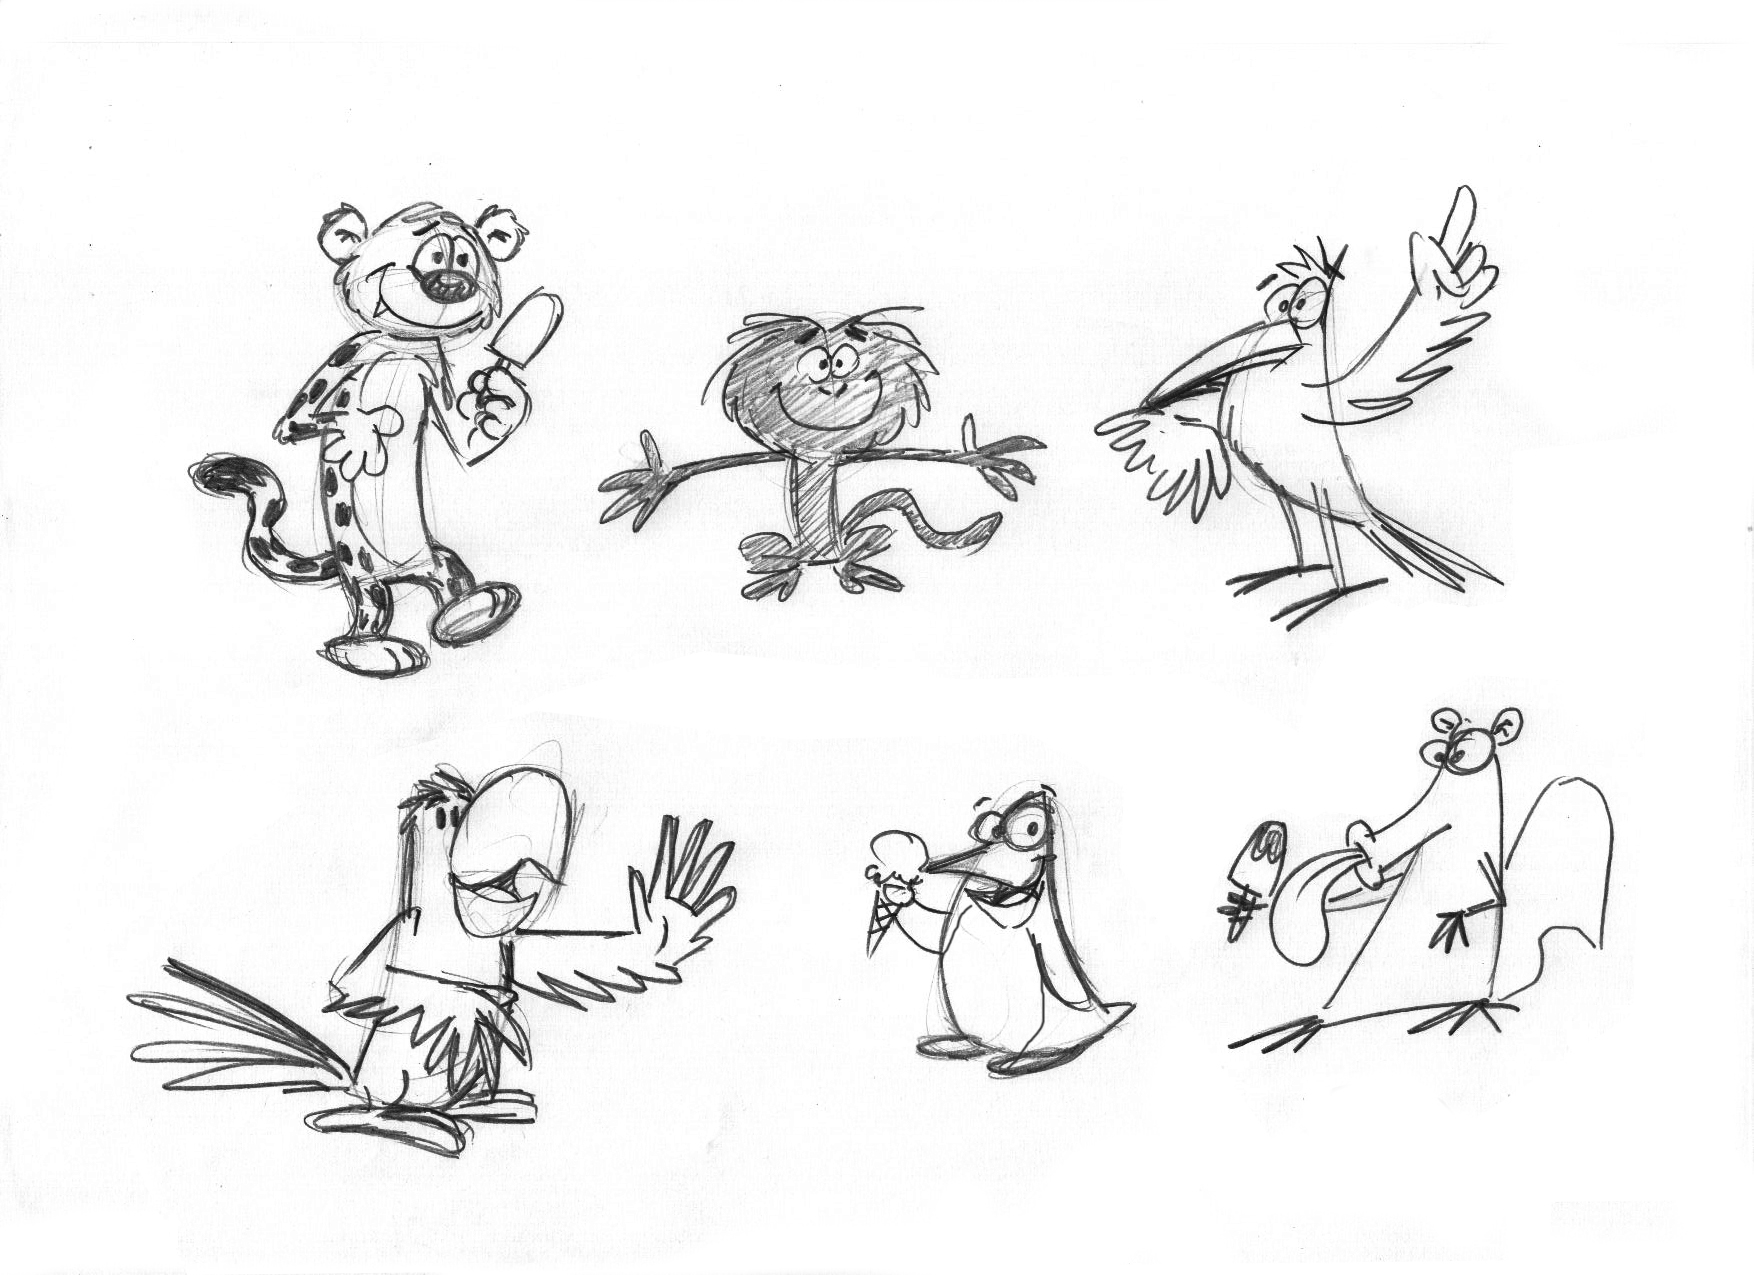
\includegraphics[height=13em]{06}

        \vspace{2.2em}
        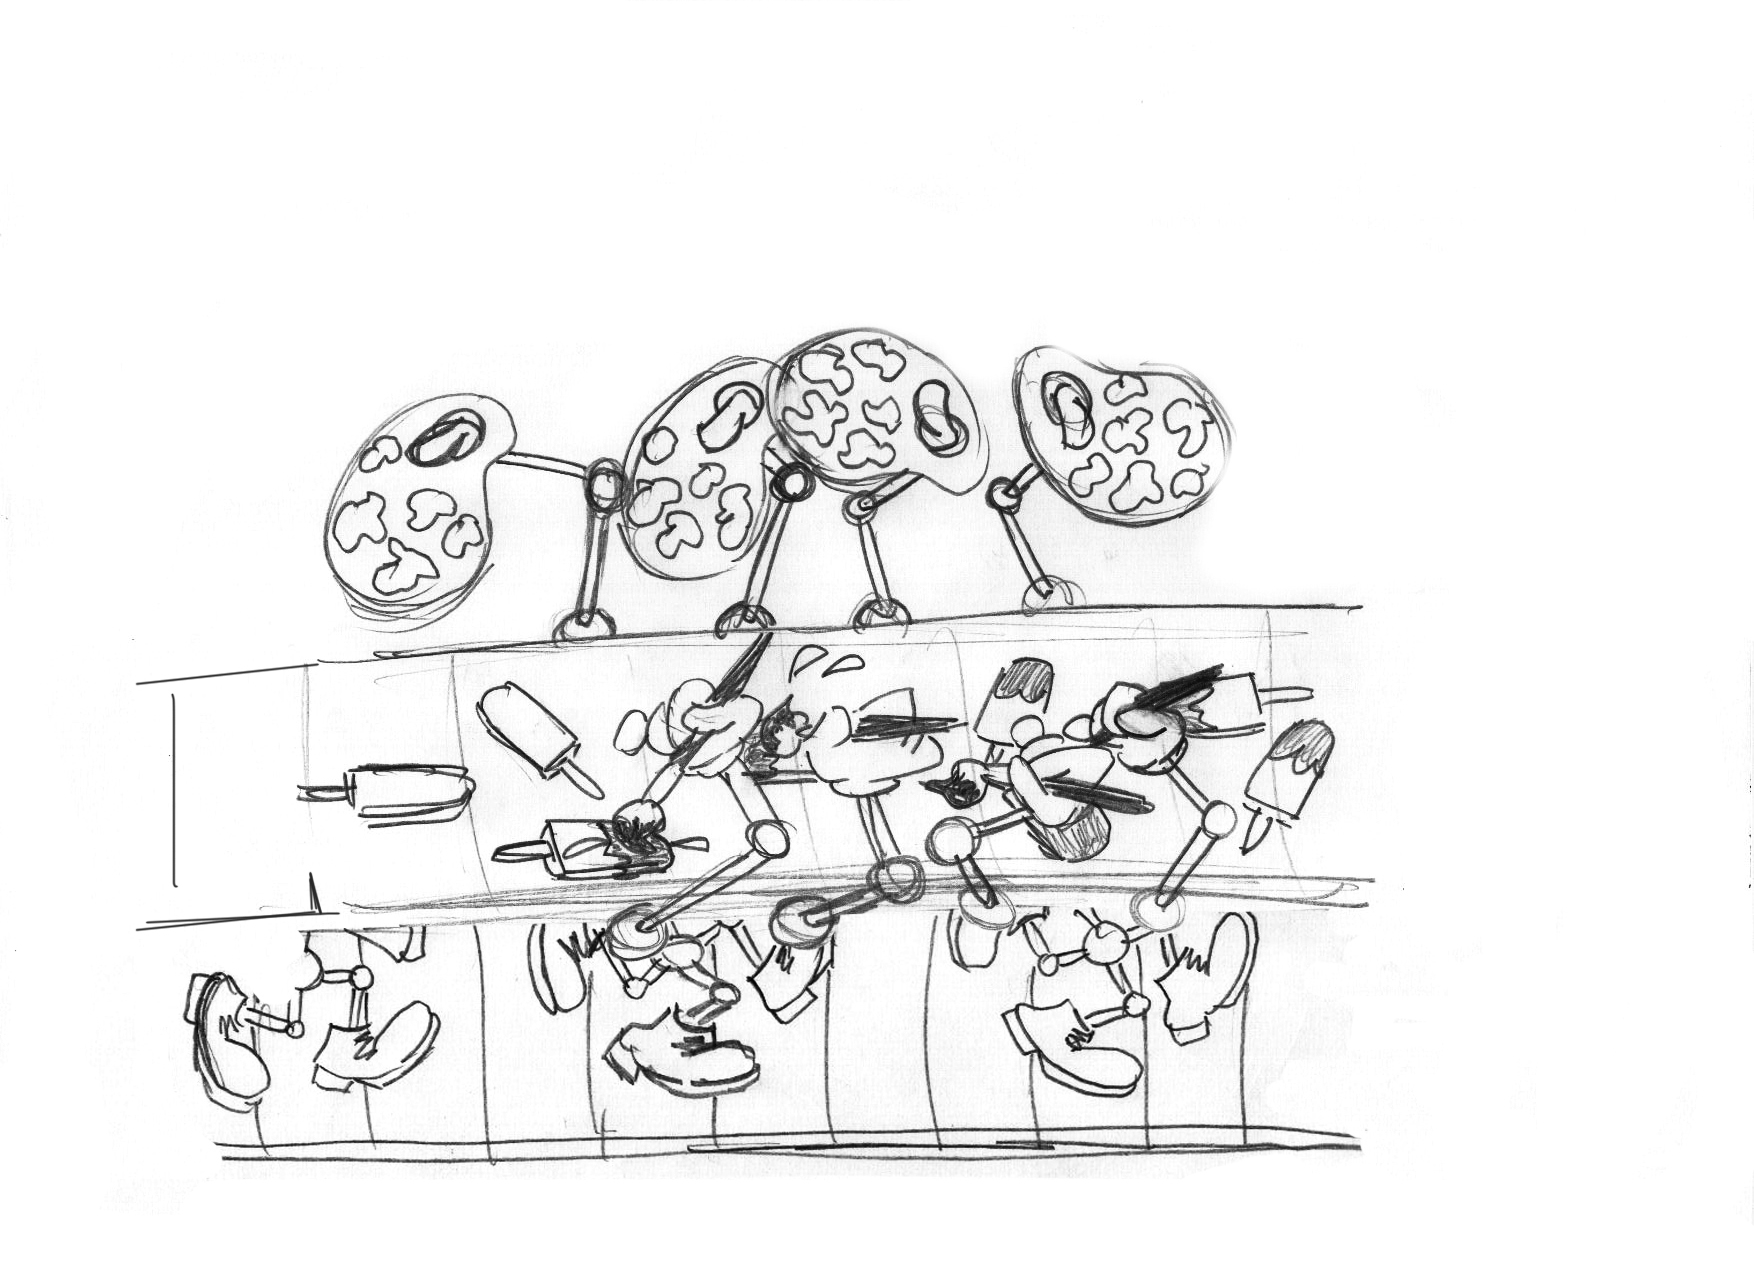
\includegraphics[height=12em]{03}
        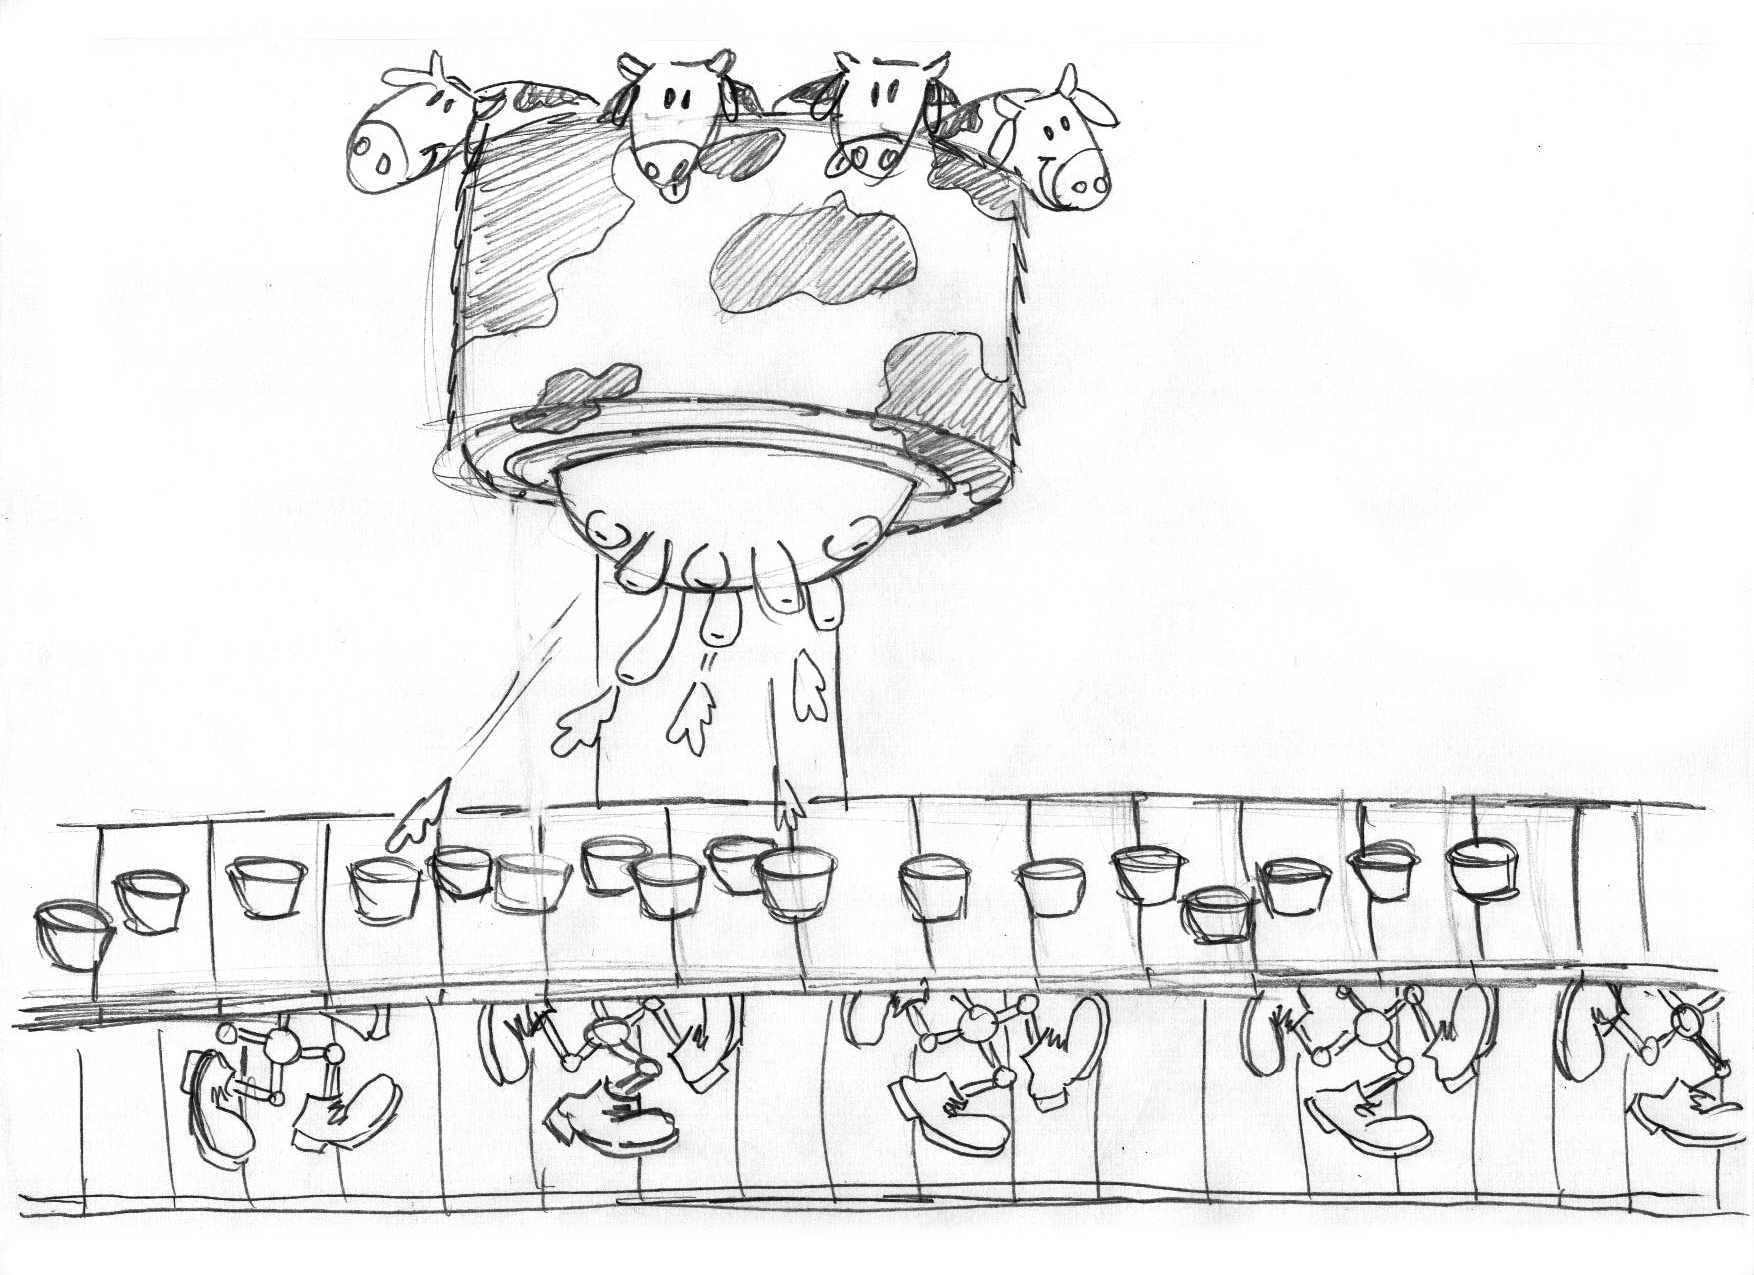
\includegraphics[height=12em]{04}
        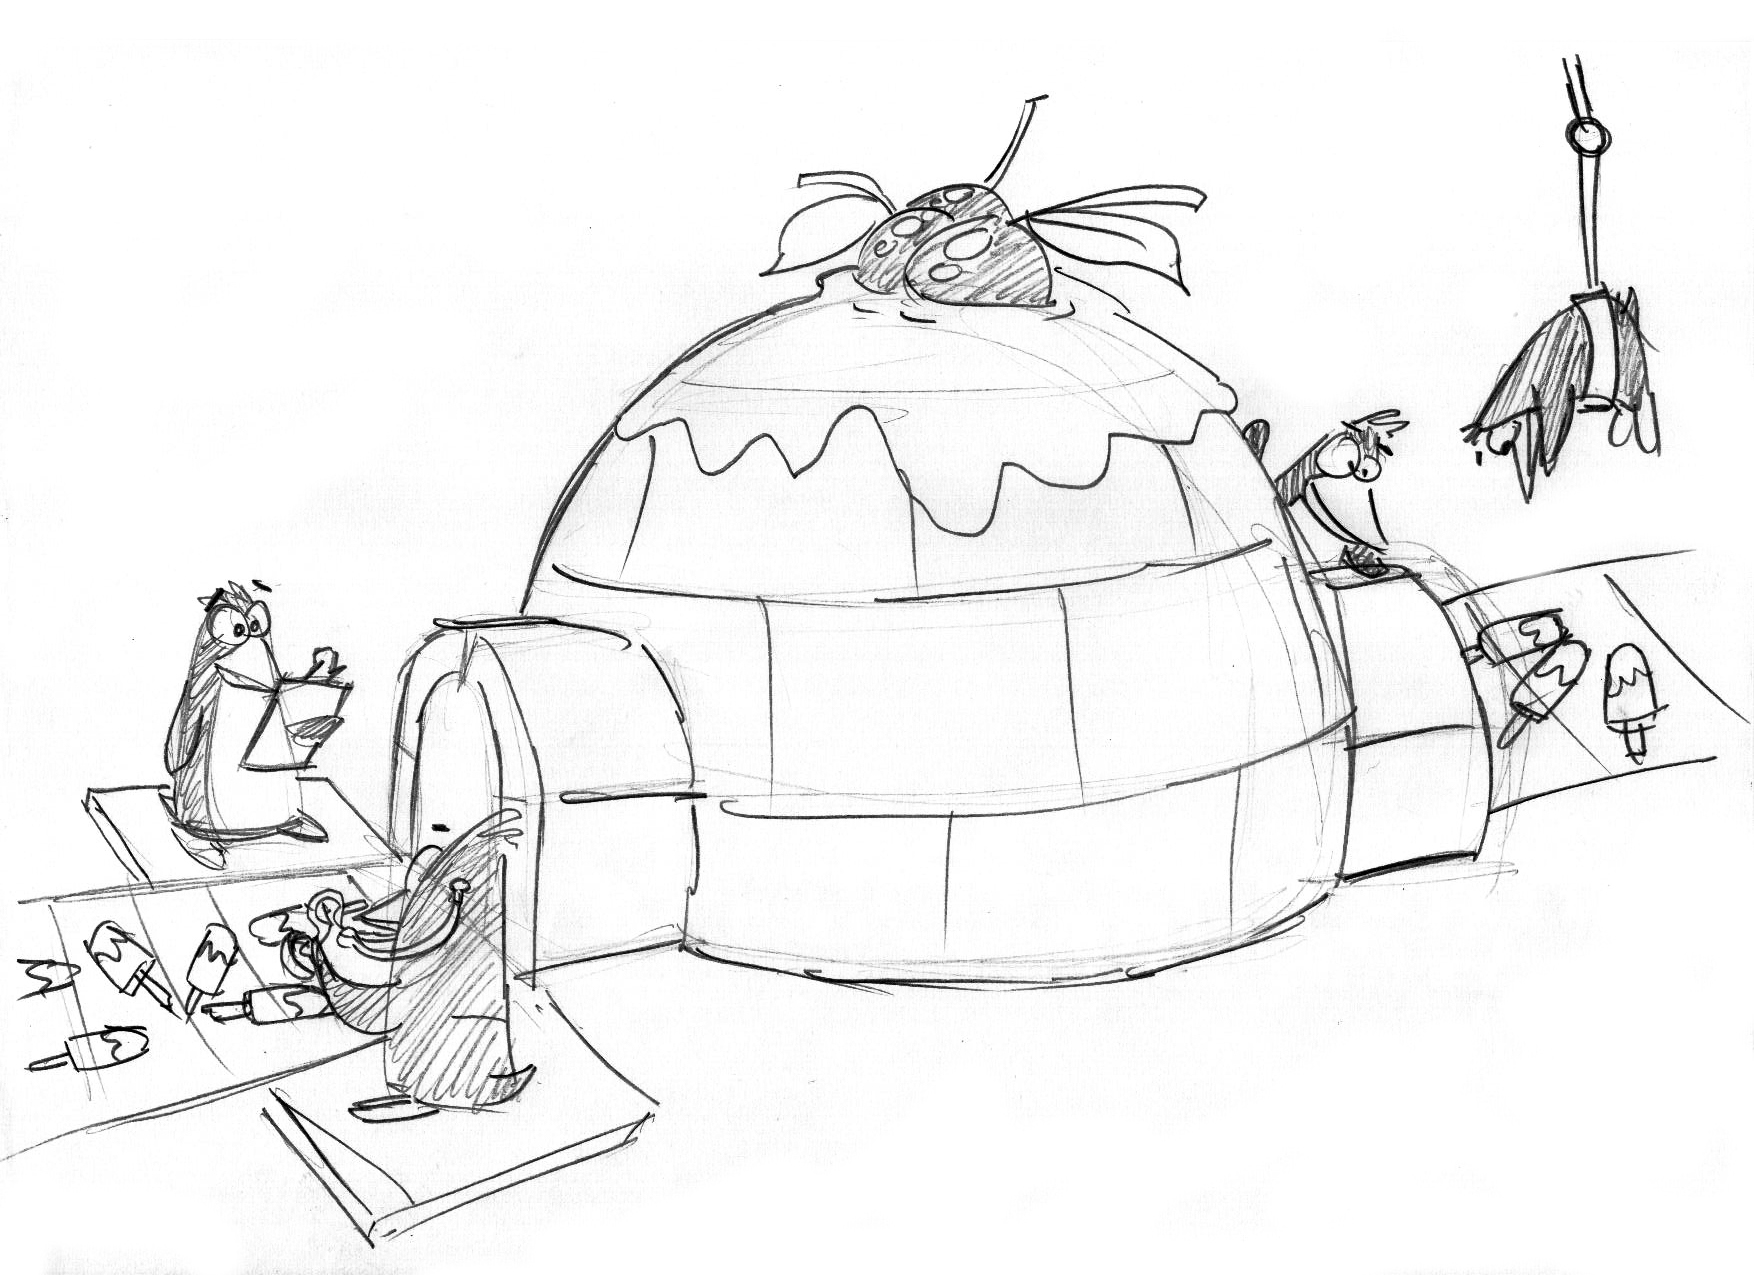
\includegraphics[height=12em]{05}

        \caption{Images from concept art.}
        \label{fig:conceptart}
    \end{figure*}

    Once the production line is set-up by, the player can start the factory and
    watch the production happening. A truck driver character provides the player
    with the customer requests and awaiting for the products, giving feedback on
    the success or failure of the puzzle.

    When the factory is running, empty cups are put in the conveyor belt by the
    cup dispenser and are carried by the conveyors in their indicated roll
    direction. When the cups get under other equipment they are manipulated by
    the intended action: for example, when under a flavor doser a scoop of ice
    cream is dispensed. Therefore, the player needs to put the devices on the
    conveyor belt \textit{in the correct order} so a specific type of ice cream
    is gradually composed. For instance, a chocolate with nuts ice cream can be
    produced by first conducting the empty cup under the chocolate flavor doser
    and then under the nuts topping doser, finally delivering it to the end of
    the conveyor belt to the truck driver.

    The puzzle difficulty increases with each level. Customers may request ice
    creams with more than one scoop or with extra toppings, which will require
    conducting the cups under a given device more than once. Also, the order
    posted by the truck driver may require different numbers of ice cream types
    (1 nuts-chocolate and 2 plain-chocolate, for instance). Additionally, the
    conveyors will form increasingly more complex shapes, requiring careful
    planing and experimentation for positioning the available equipment to
    properly satisfy the customer orders.

    The game targets both male and female players with at least 10 years old,
    without an upper limit of age.

\section{Educational Aspects Addressed}
    A problem with the existing approaches using entertainment to motivate
    learning programming skills is that they are too focused on direct input of
    code.
    \begin{quotation}
        \noindent
        \textit{The ``everyone should learn to code'' movement [...] assumes
                that coding is the goal. Software developers tend to be software
                addicts who think their job is to write code. But it's not.
                Their job is to solve problems.} \cite{Atwood2012}
    \end{quotation}

    When that focus on codding is not present, programming games are typically
    based on controlling a character's movements - such as in \doctorgame or
    \lightbot. But this approach has some constrains and tend to not embrace
    problems which require conditionals to be solved.

    The main goal of \gamename is not to teach how to write code, but instead to
    promote the development of the ground skills listed below, which are useful
    for solving computational problems.
    \begin{itemize}[noitemsep,topsep=0pt,parsep=0.75em]
        \item Consequences of operations order;
        \item How conditionals switches work;
        \item The necessity of loops and how to use them;
        \item Follow the execution steps, understand where are pieces
              causing undesired behavior, and correct that (debug).
    \end{itemize}

    Thereby we expect the players to understand more easily the structure of
    algorithms and the process of building them. So in an after moment, when a
    procedural programming language were presented, players would already have a
    more structured mind set and hopefully would feel familiar with that way of
    thinking.

    Other characteristic this kind of puzzle game has which is very interesting
    from the educational point of view is the opportunity of learning through
    trial and error. Contrary to traditional exams, which punish the students
    who are not able to get the right answer straight away, programming usually
    involves many iterations of codding, testing, and fixing. In \gamename the
    same process can applied to solve each level.

    As secondary goal, we expect the players to get familiar with a few animals
    from Brazilian fauna (the truck drivers) and with the location of some
    important cities in Brazilian map.

\section{Concept Art}
    The visual identity of \gamename is cartoonish and funny. In Figure
    \ref{fig:conceptart} there are some sketches of the art planned for the
    conveyors, devices, and characters.

\section{Acknowledgments}
    The authors would like to thank CAPES (\textit{Coordena\c{c}\~ao de
    Aperfei\c{c}oamento de Pessoal de N\'ivel Superior}) and CRI (Center for
    Research and Interdisciplinarity) for the financial support, and the artists
    Danilo Gabriel Rios and Salvador Oliva Junior for the concept art.

% Balancing columns in a ref list is a bit of a pain because you
% either use a hack like flushend or balance, or manually insert
% a column break.  http://www.tex.ac.uk/cgi-bin/texfaq2html?label=balance
% multicols doesn't work because we're already in two-column mode,
% and flushend isn't awesome, so I choose balance.  See this
% for more info: http://cs.brown.edu/system/software/latex/doc/balance.pdf
%
% Note that in a perfect world balance wants to be in the first
% column of the last page.
%
% If balance doesn't work for you, you can remove that and
% hard-code a column break into the bbl file right before you
% submit:
%
% http://stackoverflow.com/questions/2149854/how-to-manually-equalize-columns-
% in-an-ieee-paper-if-using-bibtex
%
% Or, just remove \balance and give up on balancing the last page.
%
\balance

\bibliographystyle{acm-sigchi}
\bibliography{igamer_bib}
\end{document}
